%PART_2_CHAP_4
\myChapter[érivations et autres créatures Poppy]{D}{érivations et~~\break autres créatures Poppy}\label{sec:derivation}
%WAIT a Review ok
\begin{resumChap}
Après avoir vu les différents acteurs participant à cette conception, puis  l'objet de cette conception, \cad: le robot \tiret{dans son côté physique et son côté numérique} et les ressources pédagogiques qui l'accompagnent, nous avons vu que l'un des objectifs initiaux du projet était de permettre la modification rapide et simple de la plate-forme pour l'adapter à ses besoins.\par% 
Ainsi, l'aboutissement de ce projet est de fournir un kit qui soit à la fois facile à prendre en main mais aussi permettant une forte appropriation allant jusqu'au détournement total du kit initial.\par%
Dans ce chapitre, nous verrons donc, comment certains des éléments simples de dérivation facilitent l'appropriation notamment par les possibilités simples d'ajout et de modification du kit initial.\par%
Ensuite nous traiterons de deux exemples qui illustrent ces possibilités de détournement: le projet \gui{Poppy Diplodocus} et le projet \gui{Poppy Dragster}. Le premier, réalisé par 3 élèves ingénieurs de l'ENSEIRB Bordeaux, propose une créature à pattes, et le second, par une étudiante de Master~2 \cro{Interaction Home Machine \& Design} à Stockholm (Suède) en stage de 6~mois dans notre équipe, propose une créature à roues.
\end{resumChap}
\section{Les dérivations simples et l'appropriation}
    \subsection{Nommer son robot}
        Dans un premier temps, élaborer pour des raisons techniques, \cad pour avoir plusieurs robots ErgoJr connectés sur le même réseau et répondant individuellement aux requêtes faites à l'\sht{api}\footnote{si deux robots possèdent le même \textit{hostname} et sont connectés au même réseau alors ils exécutent, tous deux simultanément, l'ensemble des instructions envoyées}, cette fonctionnalité s'est trouvée être autrement pertinente
        Nous avons fait dans un second temps, le choix de favoriser cette démarche de \cro{nommer son robot}, ceci afin d'améliorer l'appropriation et la familiarisation avec l'objet robotique. Car, on sait que nommer ses objets, plantes, voitures, et autres artefacts du quotidien nous rapproche d'eux, cependant, ce type de mécanisme chez des objets capables d'interaction est encore mal étudié. Notamment, nous montrons dans l'une de nos études, que le fait de nommer un robot anthropomorphe n'est pas gage de proximité~\citeS{Exp:name_for_bot}.
    \subsection{Ajouter des périphériques}
        Une autre manière de s'approprier le robot ErgoJr est de lui ajouter des périphériques. Les possibilités sont nombreuses: du simple \textit{speaker} audio, à la \textit{webcam} déportée~\citeURL{CC-tictactoe}, en passant par \textit{arduino} et ses jeux de capteurs~\citeURL{GL-tictactoe} ou encore par un \textit{leapmotion}~\citeURL{GL-LeapMotion} et d'autres. Cela permet d'accroître la valeur que l'enseignant porte sur la plateforme et de renforcer son sentiment de contrôle, le motivant à approfondir ses connaissances et persévérer dans l'utilisation du robot~\citeS{sec:motiv}. Cependant, cela nécessite d'avoir une bonne connaissance des deux plateformes afin de les conjuguer.
    \subsection{Modifier la structure}
        C'est un élément d'appropriation du même ordre que la customisation par ajout de périphériques. Mais contrairement à celui ci, il est extrêmement facile à mettre en place car modifer la structure ne demande pas, en soi, de compétence particulière: il suffit de posséder un fichier \sht{STL} que l'on souhaite combiner à un des supports du robot ErgoJr et d'utiliser un logiciel de \sht{CAO}; qui sont aujourd'hui très faciles de prise en main~\citeS{sec:3D_print}.
        \paragraph{Le socle}
            Un second élément qui originellement a été sélectionné pour des raisons techniques, ou plutôt de coût, est le socle. En effet, avoir un socle complètement plat et découpé à l'imprimante laser, permet de réduire les coûts de production et de stockage.
            Puis dans un second temps, nous avons constaté qu'après une phase de découverte, la majorité des utilisateurs, modifie le socle de base, trop instable. Car effectivement dès que le robot se trouve être en mouvement, ce socle, trop léger \etou pas assez large, laisse facilement basculer le robot. Le première réflexe est de tenir ce socle~\citeF{fig:Chamboule_tout}. Mais très vite le besoin de le fixé sur une surface plus adaptée devient indispensable, comme dans le projet basket proposé par Y.Bouchemoua~\citeF{fig:YB-ErgoJr-ErgoSr}. La création du socle pouvant être en soi une activité comme dans le projet proposé par C.Casseau~\citeF{fig:socle}. 
        \begin{figure}[!h]
        \hfill
        \begin{minipage}{0.3\linewidth}
            \centering
            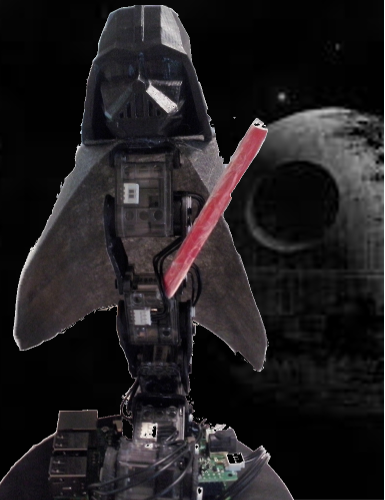
\includegraphics[width=0.9\linewidth]{Figures/ergo-dark.png}
            \subcaption{Dark Vador~\citeURL{RN-dark}}\label{fig:ergo-dark}
        \end{minipage}
        \hfill
        \begin{minipage}{0.3\linewidth}
            \centering
            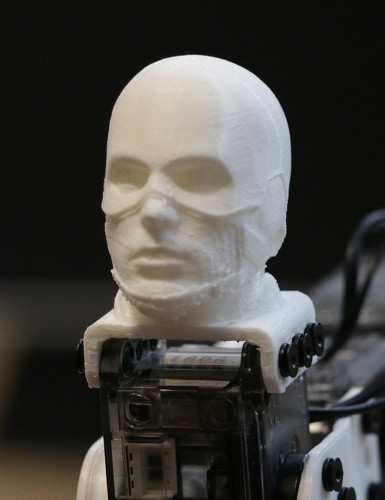
\includegraphics[width=0.9\linewidth]{Figures/ergo-captain.jpg}
            \subcaption{Captain America~\citeURL{SI-captain}}\label{fig:ergo-captain}
        \end{minipage}
        \hfill
        \begin{minipage}{0.3\linewidth}
            \centering
            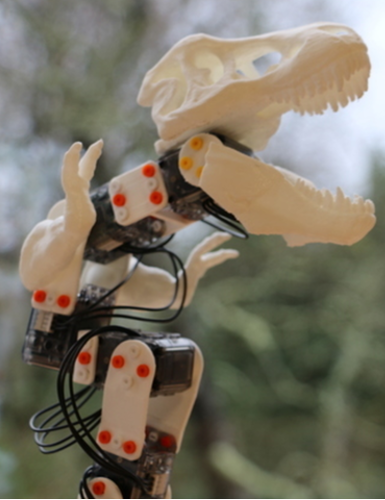
\includegraphics[width=0.9\linewidth]{Figures/ergo-sorus.png}
            \subcaption{T-Rex~\citeURL{TD-trex}}\label{fig:ergo-sorus}
        \end{minipage}
        \hfill
        \caption{Personnalisation de Poppy ErgoJr}
        \end{figure}{}
        \paragraph{Le \textit{end effector}} 
            Une modification, moins courante mais, que nous avons pu constater concerne l'embout terminal du robot aussi appelé, \textit{end effector}. Cette modification semble avoir deux origines: \Li modifier la structure pour répondre à une contrainte liée à l'objectif de la tâche à résoudre~\citeF{fig:ball-luncher} ou la tâche en elle-même~\citeURL{TD-maze}, \ii un objectif esthétique de personnalisation.
\section{Créer sa créature}
    \subsection{Recensement des projets tiers}
        De la même façon qu'il est difficile de retracer l'ensemble des utilisateurs de la plateforme~\citeS{sec:map}, il est difficile de retracer tous les projets existants. 
        Nous pouvons noter les designs de créatures de Jonathan Grizou~\citeURL{JG-crea} (ancien membre de l'équipe Flowers) ou les réalisations de Julien Jhel~\citeF{fig:quattro} et Thomas Peyruse~\citeS{sec:makers}. Durant son stage à Inria, Tallulah Gilliard proposa une classification de ces créatures~\citeB{gilliard:hal-02154848}, classification inspirée par celle de Ben-Ari~\citeF{fig:Classification}.
        \begin{figure}[!h]
          \centering
          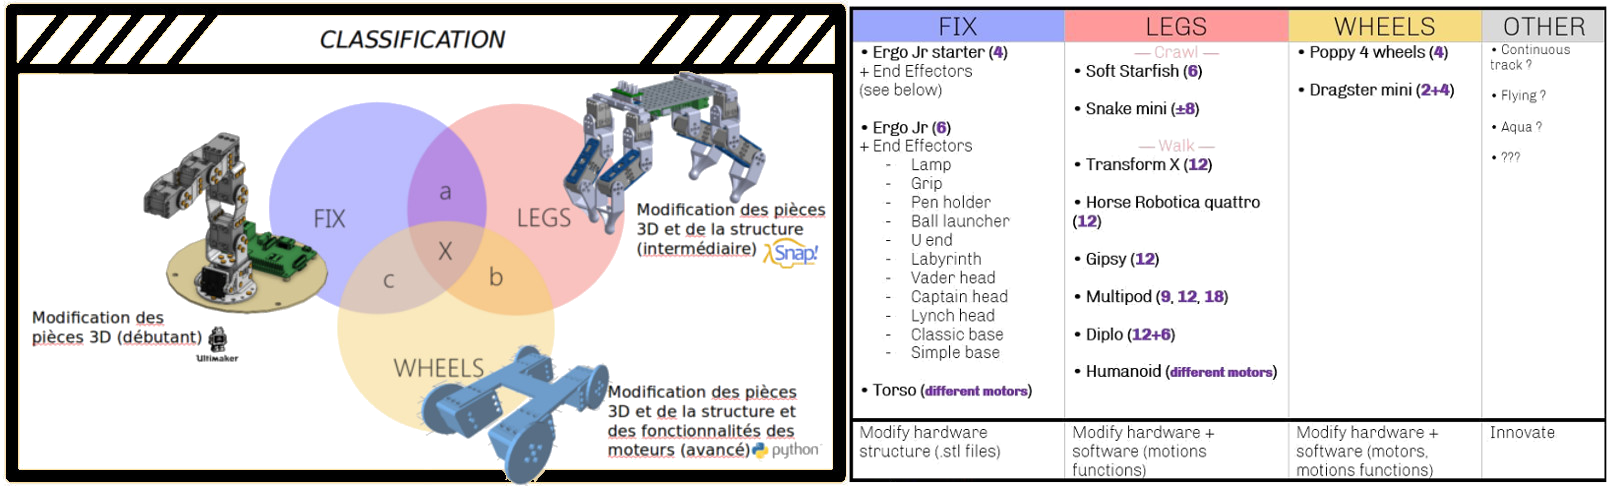
\includegraphics[width=\linewidth]{Figures/Poppy-Classification_large.png}
          \caption{Classification robot Poppy~\citeB{gilliard:hal-02154848}}\label{fig:Poppy-Class}
        \end{figure}\par%
        Pour les robots fixes, il est possible de modifier la structure (pièces 3D) sans modifier le code. Son apparence peut alors être modifiée à l'aide de logiciels de conception assistée par ordinateur, ce qui, \textit{in-fine} pourra modifier son comportement.
        Pour les robots à jambes et à roues, la modification du code source est nécessaire car une structure différente affectera leurs fonctions élémentaires.
        Des combinaisons de combinaisons telles que \cro{fixe + jambes}, \cro{fixe + roues} ou même \cro{fixe + roues + jambes} sont également possibles.
        Durant ce stage, elle participa activement au développement d'une créature alternative au robot ErgoJr: Poppy Dragster~\citeS{sec:dragster}. Cette créature fait partie des deux créatures développées dans le cadre de projet d'étude d'élèves en études supérieures.
    \subsection{Projets Étudiants}
        \begin{figure}[!h]
        \begin{minipage}{0.29\linewidth}
          \centering
          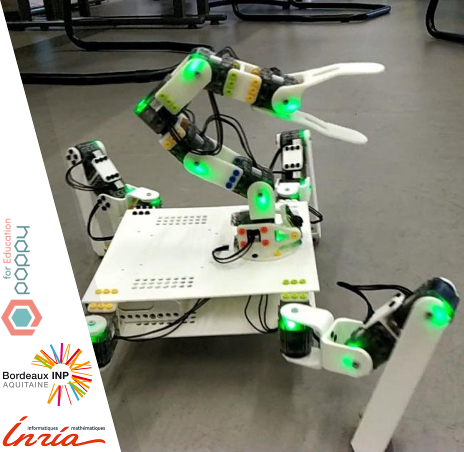
\includegraphics[width=\linewidth]{Figures/poppy-diplo}
          \subcaption{Poppy-Diplo}\label{fig:Poppy-Diplo}
        \end{minipage}
        \hfill
        \begin{minipage}{0.29\linewidth}
          \centering
          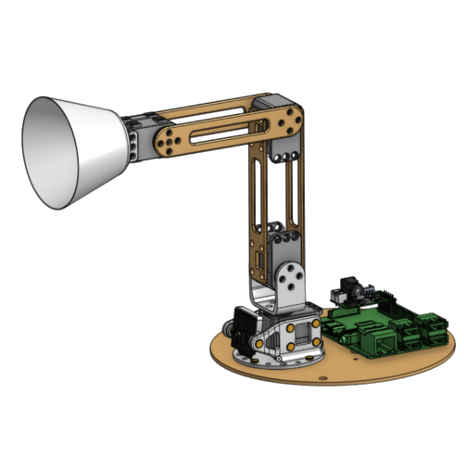
\includegraphics[width=\linewidth]{Figures/Poppy-Starter.png}
          \subcaption{Poppy-Starter}\label{fig:Poppy-Starter}
        \end{minipage}
        \hfill
        \begin{minipage}{0.38\linewidth}
          \centering
          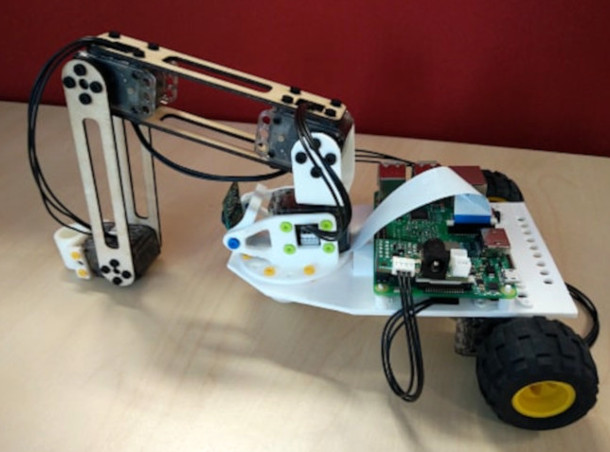
\includegraphics[width=\linewidth]{Figures/Poppy-dragster}
          \subcaption{Poppy-Dragster, Gilliard~\citeB{gilliard:hal-02154848}}\label{fig:Poppy-Dragster}
        \end{minipage}
        \caption{Dérivation et alternative à Poppy ErgoJr}
        \end{figure}
        \paragraph{Poppy Diplo}\label{sec:diplo}
            Le but de ce projet est de construire un nouveau robot qui soit capable de se déplacer, avec pour base 3 kits ErgoJr. Le projet était libre, et parmi l'ensemble des moyens de locomotion terrestres traités par les étudiants, c'est celui basé sur des pattes qui est, selon eux, le plus à même de correspondre à ce projet de robot mobile. Celui-ci permet la création d'un robot basé sur 3 kits ErgoJr avec peu d'impression de pièces 3D supplémentaires.
            L'objectif principal de ce projet était de permettre aux enseignants, disposant déjà de kits ErgoJr, de renouveler leurs enseignements en produisant une nouvelle créature à partir de ces kits. Il fallait également l'intégrer à la plateforme Poppy afin que les utilisateurs puissent reproduire la créature et l'utiliser comme ils le font habituellement avec les autres créatures de la plateforme. Pour cela, un guide permettant de reproduire le robot a été fourni.\par%
            Les objectifs ont été remplis par la création de la créature nommée Diplo qui est capable de se déplacer en avant et de tourner à droite et à gauche. L'intégration sur la plateforme Poppy est assurée par les éléments disponibles sur le GitHub du projet. Le guide d'assemblage qui contient: \Li le matériel et les composants additionnels nécessaires; \ii les programmes supplémentaires permettant le contrôle des déplacements; \iii la notice d'assemblage du robot permettant sa construction et sa mise en route.
            En suivant l'ensemble du guide, n'importe quel utilisateur disposant du matériel et des composants peut construire cette créature de manière fonctionnelle. La créature est manipulable via des primitives accessibles dans \sht{snap} ou bien par l'utilisation de fonctions Python qui sont modifiables à la guise de l'utilisateur.
            Une classe python \texttt{DiploLeg} a été créée afin de pouvoir instancier un ensemble de pattes, bénéficiant de primitives permettant d'imposer les angles de leurs moteurs \tiret{modèle direct}, ou bien d'imposer les coordonnées de leur extrémité \tiret{modèle inverse}\citeS{sec:mob_patte}.
            Le projet est en open source, il est donc possible à quiconque de le reprendre pour l'utiliser mais aussi pour l'améliorer.\par%
            \begin{table}[!h]
                \centering
                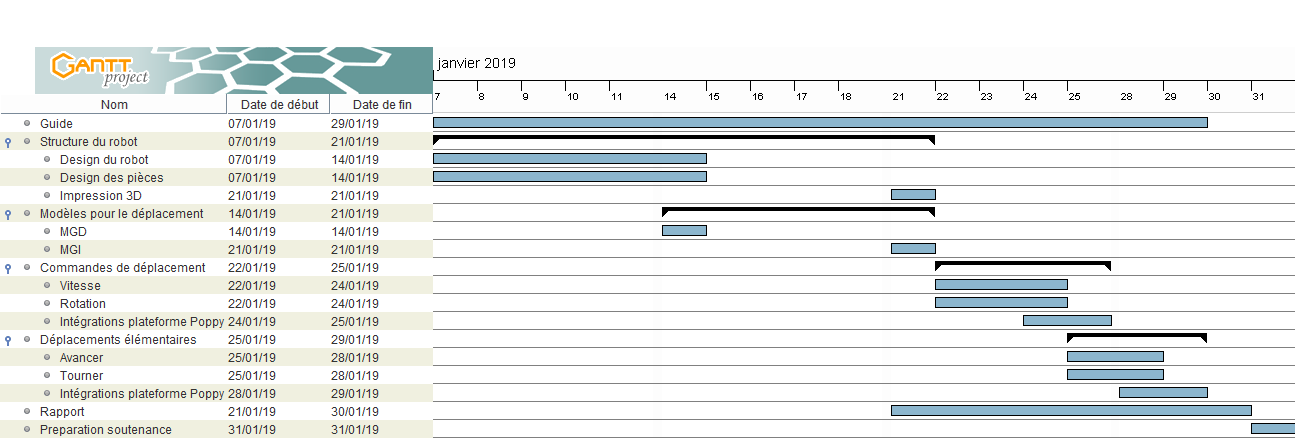
\includegraphics[width=\linewidth]{Figures/Diplo-Planning}
                \caption{Planning de réalisation Poppy Diplo}\label{tab:diplo_plan}
            \end{table}\par%
            Ce projet a été réalisé par 3 étudiants de l'ENSEIRB-MATMECA de Bordeaux: Nina Docteur, Alexis Juven et Vincent Leconte, en 3\ieme année Informatique option Robotique, durant le mois de janvier 2019~\citeT{tab:diplo_plan}. À noter qu'un État de l'art et un cahier des charges avaient été constitués au préalable et que 3 séances de 3h ont été mises en place pour la prise en main de la plateforme (construction,  installation  et  manipulation).
            Ce projet à valeur de \sht{poc} et n'a pas donné suite à d'éventuelles expérimentations.
        \paragraph{Poppy Dragster}\label{sec:dragster}
            Le Poppy~Dragster est un bras ErgoJr Starter~\citeF{fig:Poppy-Starter} composé de 4 moteurs fixés sur une plate-forme à 2 roues. L'objectif est de le rendre accessible aux personnes qui possèdent déjà un ErgoJr afin de pouvoir le transformer en un Dragster réutilisant simplement les moteurs et imprimant en 3D certaines pièces. Selon l’outil utilisé, il est capable de saisir, de tenir ou de lancer des objets, mais il est également capable de rouler en avant, en arrière et de tourner. Différentes activités peuvent alors être réalisées: détection d'obstacles, apport d'objets, schémas de dessin, \etc.\par%
            Les deux premières semaines du stage, réalisé par Tallulah Gilliard ont été consacrées à la compréhension de la plateforme et de l'environnement Poppy afin de générer des versions alternatives au Poppy ErgoJr déjà existant.\par%
            %elle commencé par quelques séances de brainstorming où j'ai essayé de penser les variations de manière large, sans restrictions. J'ai généré plusieurs modèles idéalisés et des prototypes existants et, à un moment donné, les regrouper dans une classification semblait être pertinent.
            %Comme dans d’autres disciplines de la conception, les esquisses sont largement utilisées aux premières étapes du développement de TUI \cite{buxton2010sketching}. Ils permettent de générer, d'explorer et d'expérimenter des idées, des facteurs de forme, l'expérience utilisateur et les relations possibles entre des objets d'interaction physique.
            Ensuite, c'est en combinant une structure fixe (ErgoJr Starter) et une structure de roues qu'a été créé le Poppy~Dragster
            %deux structures de robot qu'a été créé le Poppy~Dragster: il s'agit d'une combinaison d'une structure fixe (ErgoJr Starter) à une structure de roue.
            Les fichiers 3D \sht{STL} ont été créés avec TinkerCAD~\citeS{sec:3D_print} en réutilisant les formes déjà existantes du ErgoJr ou en créant de nouvelles formes à partir des formes simples. Le Dragster étant un robot à roues, il nécessitait des jantes pour fixer les roues afin que leurs formes correspondent aux dimensions (roues \textit{Lego}). La base devait supporter le bras du robot (fixé à l'avant), la Raspberry~Pi, les moteurs des roues et, éventuellement, des batteries (en option sur le robot).\par%
            Initialement, le robot ErgoJr n’était pas conçu pour avoir des roues, de sorte que tous les moteurs ont des angles limités afin de ne pas forcer le bras robotique dans une position extrême qui le casserait. Plusieurs paramètres du code devaient être adaptés à cette situation.
            \begin{code}
                \begin{minipage}{0.425\linewidth}
                    \begin{lstlisting}[language=json,basicstyle=\small]
"wl": {
      "offset": 0.0,
      "type": "XL-320",
      "id": 5,
      "wheel_mode": true,
      "orientation": "direct"
    },
                    \end{lstlisting}
                    \subcaption{\label{cod:wl}Configuration moteur roue Dragster}
                \end{minipage}
                \begin{minipage}{0.55\linewidth}
                    \begin{lstlisting}[language=json,basicstyle=\small]
"m1": {
      "offset": 0.0,
      "type": "XL-320",
      "id": 1,
      "angle_limit": [-90.0, 90.0],
      "orientation": "direct"
    },
                    \end{lstlisting}
                    \subcaption{\label{cod:m1}Configuration moteur ErgoJr}
                \end{minipage}
                \caption{\label{cod:mot_conf}Configurations par défaut des moteurs (json)}
            \end{code}\par%
            Les moteurs sont réglés différemment selon qu'il s'agit de joints de bras (m1, m2, m3, m4) ou de roues (w1, w2)~\citeC{cod:mot_conf}. Les joints dépendent d'un angle limite (entre  -90$^{\circ}$ and 90$^{\circ}$), tandis que les roues n'ont pas d'angle limite, car elles peuvent pivoter indéfiniment dans un sens ou dans l'autre. Ce code peut être facilement modifié à l’aide de l’interface Pypot de Jupyter Notebook .\par%
            Pour configurer les moteurs correctement lorsque le robot est utilisé pour la première fois, certaines lignes de commandes sont nécessaires.\par%
            Via un terminal, accessible via l’interface Jupyter Notebook, la ligne de commande \textit{poppy-configure ergo-jr m1} permet de flasher le moteur \cro{m1} en utilisant la configuration fournie par le json~\citeC{cod:m1}.
            Tous les moteurs doivent être flashés pour fonctionner et pouvoir faire démarrer le robot. Le code~\ref{cod:mot_conf_pyt} génère la commande permettant de flasher un moteur spécifique. Dans le cas des roues, le code~\ref{cod:mot_conf_wheel} a été ajouté dans le code source pour gérer sa spécificité.
            \begin{code}
                \begin{lstlisting}[language=Python]
motor_config = c['motors'][args.motor]
args = [
    '--id', motor_config['id'],
    '--type', motor_config['type'],
    '--port', find_port_for_motor(c, args.motor),
    '--return-delay-time', 0
]

if 'wheel_mode' in motor_config.keys():
    args.extend(('--wheel-mode', motor_config['wheel_mode']))
else:
    args.extend(('--angle-limit', motor_config['angle_limit'][0], motor_config['angle_limit'][1], '--goto-zero'))
                \end{lstlisting}
                \caption{\label{cod:mot_conf_pyt}Commande de configurations moteurs (pyhon)}
            \end{code}\par%
            \begin{code}
            \begin{lstlisting}[language=Python]
# Set wheel Mode
if args.wheel_mode == True:
    print('Set wheel mode')
    with DxlIOPort(args.port) as io:
        io.set_control_mode({args.id:'wheel'})
            time.sleep(.5)
        check(io.get_control_mode([args.id])[0] == 'wheel',
              'Could not set wheel Mode')
        for speed in range(0,500,10):
            io.set_moving_speed({args.id:speed})
            time.sleep(.1)
        for speed in range(0,525,25):
            io.set_moving_speed({args.id:500-speed})
            time.sleep(.1)
    print('Done!')
            \end{lstlisting}
            \caption{\label{cod:mot_conf_wheel}Configuration \cro{wheel mode} (pyhon)}
            \end{code}\par%
            Une fois le robot prêt, les pièces imprimées, les moteurs configurés et fonctionnels, aucune entrée supplémentaire n'était nécessaire pour commander le moteur: la manipulation du registre \cro{moving\_speed} était suffisante, cependant un bloc \sht{snap} spécifique a été ajouté afin de rendre l'utilisation de cette nouvelle fonctionnalité plus explicite.
            \begin{code}
                \centering
                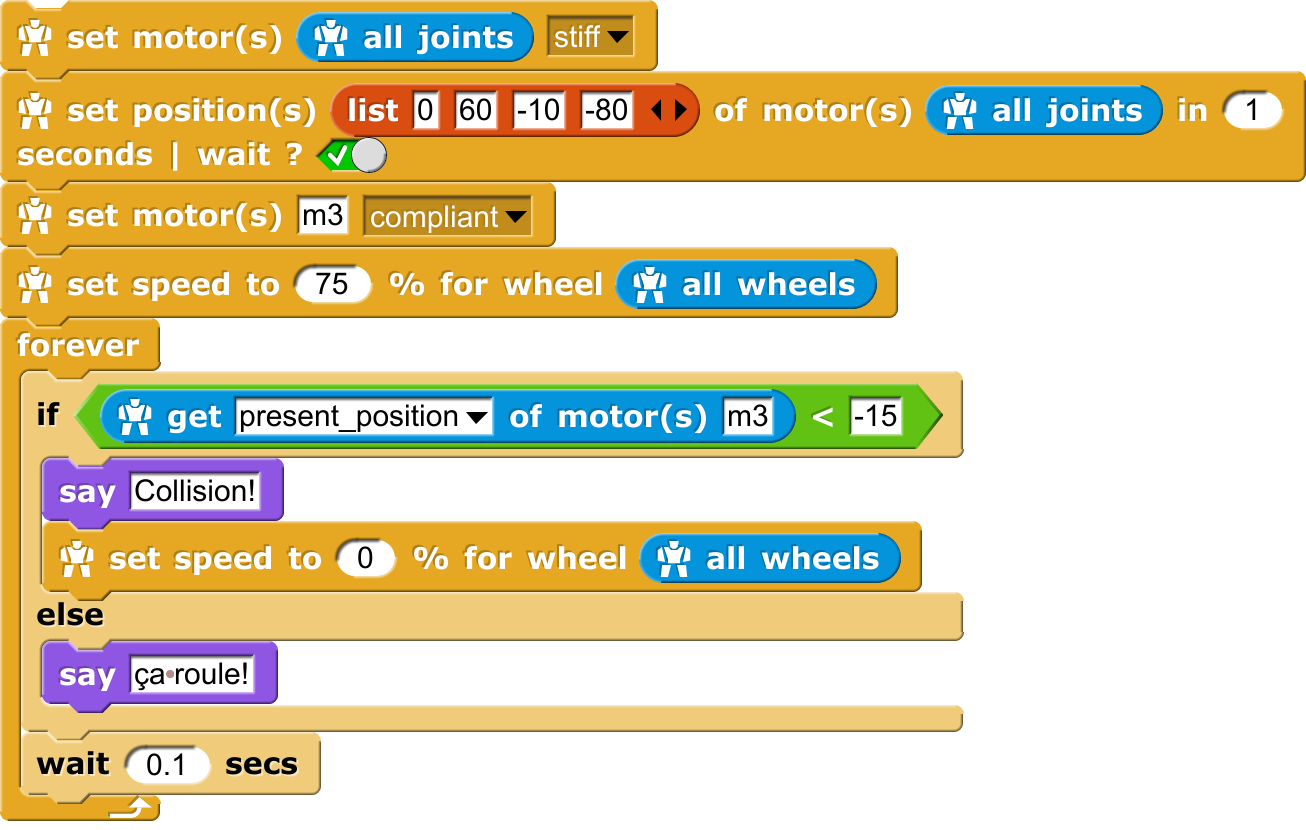
\includegraphics[width=0.75\linewidth]{Figures/Dragster_soluce}
                \caption{Solution défi, activité Dragster}\label{cod:drag_soluce}
            \end{code}\par%
            Ensuite, une activité d'initiation, similaire à celle fournie pour ErgoJr~\citeS{sec:activite}, a été développée: les utilisateurs (étudiants, enfants et débutants, \etc) doivent d'abord comprendre les bases de \sht{snap}, puis du robot: comment le faire bouger, prendre certaines positions, le faire avancer / reculer, comprendre les angles des moteurs et les blocs associés. Enfin, vient le défi: détecter un obstacle, sans recourir à la \textit{webcam}. L'astuce est de se servir du bras surplombant le dragster comme d'une canne pour aveugle. Le code~\ref{cod:drag_soluce} fourni la solution en \sht{snap}.\par%
            Mais avant d'utiliser son robot, l'utilisateur doit lui même le construire. Un guide d'assemblage a été réalisé afin de fournir une aide et des directives nécessaires à la construction du Poppy~Dragster. Il décrit plusieurs étapes: l'assemblage électronique, l'assemblage mécanique, la configuration du moteur et le test du robot.
            Sur la base de tests et d'essais menés avec des étudiants au cours d'une étude pilote, %il semble qu’il faut environ une heure pour assembler le robot à une personne qui n’a jamais assemblé un robot Poppy auparavant.
            deux variantes de ce guide ont été développées et testées~\citeS{Exp:dragster}. La 1\iere{} proposait, à des groupes de 3 élèves, un guide entièrement linéaire avec des instructions impératives; la 2\nd{} proposait une version modulaire avec des instructions formulées sous forme de conseils.\par%
            Contre toute attente~\citeF{fig:result_dragster}, c'est avec la version modulaire que les sujets se sont sentis le plus contraints (moins libre de leurs choix). Cependant, comme attendu, le partage des tâches dans cette formule, était plus aisé à mettre en place réduisant ainsi le temps de construction. D'avantage de détails sur ces résultats sont fournis en section~\ref{Exp:dragster}.